\documentclass[twoside,11pt]{article}

% Any additional packages needed should be included after jmlr2e.
% Note that jmlr2e.sty includes epsfig, amssymb, natbib and graphicx,
% and defines many common macros, such as 'proof' and 'example'.
%
% It also sets the bibliographystyle to plainnat; for more information on
% natbib citation styles, see the natbib documentation, a copy of which
% is archived at http://www.jmlr.org/format/natbib.pdf

\usepackage{jmlr2e}
\usepackage{braket}
\usepackage[]{algorithm2e}
\usepackage{multirow}
\usepackage{mathrsfs}
\usepackage[Symbol]{upgreek}
\usepackage{mathtools}
\usepackage{fancyref}
\usepackage{graphicx}
%\usepackage{placeins}
\usepackage{subcaption}
\usepackage{fixltx2e}
% Definitions of handy macros can go here

\newcommand{\dataset}{{\cal D}}
\newcommand{\fracpartial}[2]{\frac{\partial #1}{\partial  #2}}

% Heading arguments are {volume}{year}{pages}{submitted}{published}{author-full-names}

\jmlrheading{1}{2000}{1-48}{4/00}{10/00}{Name and Name}

% Short headings should be running head and authors last names

\ShortHeadings{Imitation Learning for Accelerating Fixed Point Iterative Processes }{Name and Name}
\firstpageno{1}

\begin{document}

\title{Imitation Learning for Accelerating Fixed Point Iterative Processes}
%title{Speeding up Hartree-Fock by Imitation Learning}

\author{\name Name\ Name \email email \\
       \addr Department\\
       University \\
       City, State , USA
       \AND
       \name Name\ Name \email email \\
       \addr Department\\
       University \\
       City, State , USA}
\editor{editor name}

\maketitle


\begin{abstract}
A means to accelerate iterative processes by using imitation learning is provided. This work focuses on the application of quantum mechanics and solving Hartree-Fock, which is a method for approximating the electron distribution and energy of a given molecular system. Hartree-Fock is excessively time-consuming or even infeasible when applied to large molecules. Besides, depending on input, it is not always guaranteed to converge to a solution. Speeding up Hartree-Fock and making it more robust would thus enable scientists to deal with more complicated molecules and study chemical reactions with larger systems. In the present work, we attempt to improve on Hartree-Fock by imitation learning: from the trajectory produced by the original Hartree-Fock, we extract an (expensive to evaluate) expert policy which converges to a solution quickly and reliably, and attempt to imitate this policy with a less-expensive policy class.  To solve the imitation learning problem, we apply the Dataset Aggregation algorithm (DAgger), which learns a policy that is guaranteed to perform well under its induced distribution of states. In the experiment, we show that after 
%applying one iteration of DAgger, we got a faster convergence. 
 multiple iterations of DAgger, the performance improves and becomes less over-fit. 
\end{abstract}

\section{INTRODUCTION}

Many computational methods in science and engineering use fixed-point iteration
\[
x_{n+1} = f(x_n), \quad n = 0,1,2,3...
\]
to attempt to find fixed points of $f$, i.e. points at which $f(x)=x$. The iterations generate a sequence, $x_0, x_1, x_2, \ldots$, that ideally converge to a fixed point, $x$. This paper explores the application of imitation learning to fixed-point iteration to accelerate convergence and improve stability. Imitation learning, also called learning from demonstration, is designed to learn a policy that imitates an expert's demonstration so as to become capable of performing the task demonstrated by the expert. For the important fixed-point problems of science and engineering, considerable effort have gone into developing and fine-tuning fixed-point iteration algorithms. The sequences generated from these existing algorithms, $x_0, x_1, x_2$  provide a basis for creating expert demonstrations with enhanced performance. For example, the series $x_0, x_2, x_4$ provides an enhanced expert demonstration with accelerated convergence. The use of imitation learning to discover policies that mimic the behavior of such enhanced experts has the potential to substantially improve algorithms that are at the core of much of computational science.


In the field of computational quantum chemistry, the Hartree-Fock method is a fixed-point algorithm that is used to approximate the electronic structure and energy of molecules. Hartree-Fock is a specific instance of a broader class of mean-field theory approaches to many-body problems. In such mean-field theories, the effect of all individuals on any given individual is approximated by a single averaged effect, thus reducing a many-body problem to a one-body problem. In quantum chemistry, the mean field arises from the averaged charge distribution of the electrons, as described by the electron density, $\rho({\bf r})$. The Hartree-Fock iterations thereby generate a series of electron densities that ideally converge to a fixed point. Quantum chemical methods that go beyond mean-field theory typically begin with the results of a Hartree-Fock calculation, making the Hartree-Fock algorithm a pervasive component of quantum chemistry.\cite{Some authoritative review of electronic-structure theory}

Here, well-established Hartree-Fock algorithms are used to generate series of electron densities from which enhanced expert demonstrations are constructed. We then apply supervised learning to train a policy that mimics the demonstration. However, naive supervised learning may yield poor performance in practice and also in theory.  Because the learner's prediction and action affect future observations and states during the execution of the learned policy, it obviously violates the common i.i.d. assumption made in most statistical learning approaches \citep{Ross}. Fortunately, the dataset aggregation algorithm (DAgger), proposed by Ross et al. \citep{DAgger}, can learn a stationary deterministic policy guaranteed to perform well under its induced distribution of states. This in turn serves as a remedy to the poor performance in naive supervised learning. DAgger also has been shown to have stable performance and fast learning rate \citep{DAggerCompare}. Below, DAgger is shown to yield policies whose performance is superior to those obtained from more naive approaches. 

\section{BACKGROUND}

\subsection{Hartree-Fock}

The core problem of quantum chemistry is to compute the electronic distribution, given the position of the nuclei. In Hartree-Fock theory, the distribution is described by the electron density, $\rho({\bf r})$, which gives the probability of finding any electron at the position ${\bf r}$. Hartree-Fock theory derives from the time-independent Schr\"{o}dinger equation,
\begin{equation} \label{eq:schrodinger}
				\hat{H}\Psi = E\Psi
\end{equation}
where $\hat{H}$ is the Hamiltonian operator and the many-body, or many-electron, wave-function $\Psi$ is an eigenfunction of that operator. Different $\Psi$'s correspond to different quantum states of the system, but the goal of Hartree-Fock theory is to approximate the lowest-energy state. [expand?]  Hartree-Fock theory uses a mean-field approach to convert the many-body Schr\"{o}dinger equation to a one-electron problem,
\begin{equation} \label{eq:fockSchrodinger}
				\hat{F}\phi_a({\bf r}) = \epsilon_a \phi_a({\bf r})
\end{equation}
where $\hat{F}$ is the Fock operator, $\phi_a({\bf r})$ are the molecular orbitals, which describe the possible quantum states of individual electrons, and $\epsilon_a$ are the molecular orbital energies. An approximation for the many-electron system is then constructed by assuming the $N$ electrons of the molecule occupy the lowest-energy orbitals, consistent with the Pauli exclusion principle restriction of placing at most two electrons (one with spin up and one with spin down) into any given molecular orbital. The Fock operator
\begin{equation} \label{eq:fock}
\hat{F}(\rho) = \hat{h}_1 + \hat{G}(\rho({\bf r}))
\end{equation}
where $\hat{h}_1$ is the one-electron Hamiltonian containing the operators that account for the kinetic energy of the electrons and the interaction of the electrons with the nuclei. $\hat{G}$ is an operator that captures the interaction between a single electron and the mean field resulting from all electrons. This mean field is constructed from the electron density, $\rho({\bf r})$. 

For computational expediency, the molecular orbitals, $\chi_a$ of Eq.~\ref{eq:fockSchrodinger} are written as a linear combination of atomic orbitals,
\begin{equation}\label{eq:lcao}
\phi_a({\bf r}) = \sum_{i=1}^{N_{basis}} \chi_i({\bf r}) C_{i,a}
\end{equation}
The set of basis functions provides a finite-dimensional Hilbert space in which to obtain approximate solutions. In this space, the operators $\hat{F}$, $\hat{h}_1$ and \hat{G}, along with the density $\rho({\bf r})$ become symmetric matrices of dimension $N_{basis}$ and Eq.~\ref{eq:fockSchrodinger} becomes a generalised matrix eigenvalue problem,
\begin{equation}\label{eq:fockMatrix}
F(\rho)C = SC\epsilon
\end{equation}
where $F$ is the Fock matrix and $S$ is the overlap matrix of inner products of the basis functions. $\rho$ is the density matrix which expresses the electron density $\rho(({\bf r})$ in the basis set and is given by $C^TC$. Hartree-Fock scales nominally as $N_{basis}^4$ due to the evaluation of $\hat{G}$, although scalings closer to $N_{basis}^3$ are routinely achieved by taking advantage of sparsity in construction of $\hat{G}$\ref{?}.


\begin{algorithm}[htb]
 \KwData{ 3D coordinates of atomic nuclei}
 \KwResult{Density matrix which gives minimum energy}
	Choose basis set of desired size \\
	Initialize $i \leftarrow	 0$ \\	
	Pick a starting density matrix $\rho_0$ \\
	Pick $\delta$ to be a small value (termination criteria) \\
 \While{ $i=0$ or $|E_{i} - E_{i-1}| > \delta$ }{
    Construct guess density matrix $\rho$ from available $\rho_i$ \\
	Calculate the Fock operator  $F \leftarrow h_1 + G(\rho)$\\
	Solve for $\epsilon$ and $C$ using Eq.~\ref{eq:fockMatrix} \\
	Update density matrix $\rho_{i+1}$ = $C^TC$\\
	$i \leftarrow i+1$ \\
 }
 \caption{Hartree-Fock algorithm}
\label{alg:hf}
\end{algorithm}

The corresponding fixed point iteration is shown in Algorithm\ref{alg:hf}. Implementations differ with regards to the means used to construct the starting density matrix and, more importantly for the current study, with regards to the means used to construct a guess density matrix from past iterates, $\rho_i$. This is typically done by taking a linear combination of these past iterates. In the Direct Inversion in the Iterative Subspace (DIIS) method\citep{Pulay1980}, the linear coefficients are chosen by associating an error vector which each iterate and choosing coefficients that minimize the summed error. Various methods have been used to define the error vector and to find the linear combinations that minimize the predicted error.~\citep{ADIIS,compScuseria,Alejandro2012} However, how to generate linear combinations that lead to the fastest convergence remains an open question\citep{Konstantin2002, Thorsten2011}. The current work retains the approach of using a linear combination of past iterates, but uses supervised learning to discover the optimal coefficients. 

\subsection{Speeding up Hartree-Fock as an imitation learning problem}

Accelerating Hartree-Fock convergence has previously been explored in the matter of creating a linear combination of the density matrices generated from previous iterations to serve as a better input to the next iteration of Hartree-Fock \citep{Pulay1980}. 


However, the issue of finding the best linear combination that may lead to the final density matrix faster still leaves room for further discussion.

In this paper,
we want to explore the linear combination that can speed up this iterative process by imitation learning. 
%This could perhaps also lead to finding a good initial guess density, which may speed this method significantly. 


%How to map the Hartree-Fock to imitation learning problem.
%As we mentioned before,  because of the Fock operator can only be calculated iteratively, Hartree-Fock approaches the steady-state density matrix iteration by iteration.

%Given an initial guessed density matrix $\rho_0$ as an input for solving Fock operator, after first iteration we will have the a new output density matrix $\rho_1$. In the following iterations, the previous output density matrix will then become the input to the next iteration. 


%This repeating process is quite tedious. If we can make each iteration more productive, we can reach the final steady-state density matrix with less iterations thus make the whole process faster.

If we think the whole $n$ iterations of the Hartree-Fock process as a sequence, beginning from initial density matrix $\rho_0$ through $n-1$ intermediate density matrices $\rho_1$,  $\rho_2$,  $\ldots$ ,$\rho_{n-1}$ and finally ending at steady-state converged output $\rho_{n}$, we indeed don't care about the intermediate density matrices. The only thing we want to know is the final steady-state density matrix. If we can get the final steady-state density matrices with fewer iterations or even one iteration of computation that would greatly shorten the computation time and thus speed up the whole process. 


% TODO:MOUNTAIN HIKING
%If we think of the sequence of density matrices as a film playing frame by frame. Then it is intuitive to think of a 2X speeding up version Under the same frame rate, the sequence of a  "2X fast forward" version would be dropping the odd numbered frames, thus the sequence will become $\rho_0$ to $\rho_2$, $\rho_2$ to $\rho_4$, \ldots $\rho_{n-2}$ to $\rho_n$. In this ideal fast forward version, we will only need half iterations to achieve the same goal, thus cutting the computation cost into half.

Assume we have a set of $n$ density matrices generated in sequence   $\rho_0 \rightarrow  \rho_1 \rightarrow  \rho_2  \ldots  $ and finally converging at $\rho_{n}$. 
We can build up a faster trajectory from this sequence and try to learn from it.
One example can be a sequence which has a step size of 2 of the original trajectory, like $\rho_0 \rightarrow \rho_2 \rightarrow  \rho_4 \rightarrow  \ldots \rightarrow  \rho_{n}$. Then for this trajectory, it only takes $\frac{n}{2}$ iterations for reaching the steady-state density matrix instead of $n$.
As a choice, we can build an even greedier trajectory that no matter what the input density matrix is, it always takes only one step for returning the steady-state density matrix ($\rho_0 \rightarrow \rho_{n}$).


These trajectories can be turned into a policy which maps every input in current step to the desired next step. With the policy serving as an expert's demonstration, we can apply imitation learning, to train a modified version of Hartree-Fock which uses the linear combination of the density matrices generated from previous iteration to serve as input mimicking the expert's demonstration extracted from base Hartree-Fock trajectory.

As a consequence, by imitation learning, it's possible to make more progress in one iteration, thus converge with fewer iterations and speed up the whole process.  

%The present work therefore intends to treat the Hartree-Fock process as an expert demonstration, and we apply DAgger algorithm to imitate the process for learning a fast-forward version of Hartree-Fock.


%if you want to use more Gaussian functions to get a more accurate description of the orbitals. 

%Hartree-Fock is a method used to get the density matrix for a given molecule. The density matrix describes the molecule and the probability distribution of the location of the electrons.

 %Hartree-Fock is an approximation for solving the Schr\"{o}dinger equation where it assumes that the wave function can be approximated by a single Slater determinant. The electrons or orbitals are described with a combination of Gaussian functions.

%Hartree-Fock
%density matrix
%Gaussian  , wave function, basis

\subsection{DAgger algorithm}
% sovle the naive imitation learning problem
DAgger is an algorithm that learns from an expert demonstration in an iterative manner. In each iteration, a model is trained under the states that were induced by both the expert and by the previous learned models. This aggregation expands the training to include inputs that the model is likely to encounter based on previous training iterations. By doing so, it is possible to offset the error made by previous learned models and thus learn a new policy that better approaches the demonstration. This is a remedy to the problem, in naive supervised learning, that the error may grow quadratically and results may become unpredictable because the policy is trained under a different state distribution than the model may encounter. 


The DAgger algorithm is given as Algorithm \ref{alg:DAgger}. $\Pi$ is the class of policies the learner is considering.
In the first iteration, it uses the expert's policy $\pi^*$ to gather
a dataset of trajectories $D$ and train a policy $\hat{\pi}_2$ that best mimics the expert on those trajectories. 

Then in iteration $i$, we sample states according to a mixture of policies ($\hat{\pi}_i$ and the expert $\pi^*$) and refer to expert's action on these states, forming the dataset $D_i$, which is in turn added to the overall dataset $D$. We then train the next policy $\hat{\pi}_{i+1}$, the policy that best mimics the expert on the whole dataset $D$. The process is then repeated to further rectify the error produced by the policy learned in the previous iteration until we reach iteration $N$.



\begin{algorithm}[htb]
 \KwData{Expert's demonstration generated by expert's policy $\pi^*$}
 \KwResult{Best $\hat{\pi}_i$ on validation }
 $\pi^*$  is the expert’s policy \\
 Initialized $D \leftarrow \emptyset$ \\
 Initialized $\hat{\pi}_1$ to any policy in $\Pi$ \\
 \For{i=1 to N }{
	Let $\pi_i$ = $\beta_{i}\pi^* + (1-\beta)\hat{\pi_i}$ \\
	Sample T-step trajectories using $\pi_i$ \\
	Get dataset $\rho_i$ = \{(s, $\pi^*$(s))\} of visited states by $\pi_i$ and actions given by expert. \\
	Aggregate datasets: $D \leftarrow D \cup \rho_i$ \\
	Train classifier $\hat{\pi}_{i+1}$ on $D$\\
 }
 \caption{DAgger algorithms}
 \label{alg:DAgger}
\end{algorithm}

% Connecting the symbol in algorithm to our scenario

%DAgger is a powerful algorithm that can train a model which performs well in its the induced state.

\section{LEARNING THE POLICY}

\begin{center} 
	\begin{table*}[t]
	\footnotesize\setlength{\tabcolsep}{2.5pt}
	\renewcommand{\arraystretch}{1.5}
		\caption{Applying DAgger on the Expert's demonstration with step size = 2}
		\begin{tabular}{|l|l|l|l|l|l|l|l|}
			\hline	& \multicolumn{7}{l|}{	Hartree-Fock iterations (with step size = 2)} \\ \hline	\multirow{10}{*}{
				\begin{tabular}[c]{@{}l@{}}DAgger\\ iterations\end{tabular}}	 
	&      iter          &                &  iter 1         & iter 2          & iter 3         & \ldots         & iter x = $\frac{n}{2}$         
	\\ \cline{2-8} 	& \multirow{2}{*}{ 1} 
	& Objective & $(\rho_0) \rightarrow \rho_2$ & $(\rho_0,\rho_2) \rightarrow \rho_4$ & $(\rho_0,\rho_2,\rho_4) \rightarrow \rho_6$ &  \ldots & $(\rho_{2i})_{i=0}^{x-1} \rightarrow \rho_{n}$ \\ \cline{3-8} 
	&                 & Result & ($\rho_0) \rightarrow \rho_2'$ & $(\rho_0,\rho_2)  \rightarrow \rho_4'$   & $(\rho_0,\rho_2,\rho_4) \rightarrow \rho_6'$    &  \ldots & $(\rho_{2i})_{i=0}^{x-1} \rightarrow \rho_{n}'$          \\ \cline{2-8} 
	& \multirow{2}{*}{ 2} & New objective         &                         & $(\rho_0,\rho_2')  \rightarrow \rho_4$   & $(\rho_0,\rho_2,\rho_4') \rightarrow \rho_6$     &  \ldots & $((\rho_{2i})_{i=0}^{x-2} ,\rho_{2(x-1)}')\rightarrow \rho_{n}$          \\ \cline{3-8} 
	&                 & Result &                 & $(\rho_0,\rho_2') \rightarrow \rho_4''$ & $(\rho_0,\rho_2,\rho_4') \rightarrow \rho_6''$   & \ldots & $((\rho_{2i})_{i=0}^{x-2} ,\rho_{2(x-1)}') \rightarrow \rho_{n}''$        \\ \cline{2-8} 
	& \multirow{2}{*}{ 3} & New objective         &                         &                          & $(\rho_0,\rho_2',\rho_4'')  \rightarrow \rho_6$    &  \ldots & $((\rho_{2i})_{i=0}^{x-3} ,(\rho_{2i}^{[i-(x-3)]})_{i=x-2}^{x-1}) \rightarrow \rho_{n}$         \\ \cline{3-8} 
	&                 & Result &                 &                 & $(\rho_0,\rho_2',\rho_4'')  \rightarrow \rho_6'''$ &  \ldots & $((\rho_{2i})_{i=0}^{n-3} ,(\rho_{2i}^{[i-(x-3)]})_{i=x-2}^{x-1})\rightarrow \rho_{n}'''$      \\ \cline{2-8} 
	& \vdots      & \vdots      &                &                &                & $\ddots$ &   \vdots \\ \cline{2-8} 
	& \multirow{2}{*}{ x=$\frac{n}{2}$} & New objective         &                         &                          &                            &  & $(\rho_{2i}^{[i]})_{i=0}^{x-1} \rightarrow \rho_{n}$     \\ \cline{3-8} 
	&                & Result  &                &                &                &  & $(\rho_{2i}^{[i]})_{i=0}^{x-1}\rightarrow \rho_{n}^{[x]}$ \\ \hline
	\end{tabular}
	\end{table*}
\end{center} 

%Our goal is to have the Hartree-Fock with linear combination achieve the same steady-state density matrix with less iterations, say, half or even less.  


% The original Hartree-Fock is actually a Hartree-Fock with all-zero embedded paramter

% In our scenario the 2X fast forward version of Hartree-Fock is \pi^*
% D is the training dataset that compose of the input density matrices and correspondent ideal output density matrices
% 

With a faster trajectory serving as the expert's demonstration, we would like to learn a policy that for each single iteration of Hartree-Fock forms the input to the next iteration from the linear combination of previous output density matrices.   

Referring to the DAgger algorithm, in our case, $\Pi$ is the policy class consisting of all modified Hartree-Fock methods augmented with linear combinations of past density matrices. $\pi^*$ represents the expert's policy that generates the expert's demonstration which can be constructed from a trajectory. 

%However, we don't need to have an explicit expert's policy, instead we can build up the the expert's demonstration with any Hartree-Fock trajectory from scratch. 

%A policy here is composed of sets of coefficients which represents the linear combination to apply in each Hartree-Fock iteration. 


% ???????????
%When applying DAgger to Hartree-Fock iteration $i$, we initialize $\pi_{(1)}$ equal to $\pi^*$. Then in during the DAgger iterations, we can generate a sequence of policies $\hat{\pi}_{(2)} , \hat{\pi}_{(3)}, \ldots, \hat{\pi}_{(i+1)}$, in which the output of previous policy will become the input of next policy.


The main idea of DAgger is to train the policy under the induced state of the previous policies. Therefore, refer to the DAgger algorithm, when training policy $\hat{\pi}_{i}$ in DAgger iteration $i-1$,
we will consider states generated from the previous policy $\hat{\pi}_{i-1}$ and all earlier policies. That is to say, if we think of each single Hartree-Fock iteration in isolation, we can denote $\hat{c}_{(i,j)}$ the set of coefficients trained in the Hartree-Fock iteration $i$ and DAgger iteration $j-1$. Then the output of the density matrices generated from $\hat{c}_{(i,j)}$ after Hartree-Fock can in turn be used to train $\hat{c}_{(i+1,j+1)}$, the set of coefficients in the next Hartree-Fock iteration in the next policy.


We can visualize the whole process as a two-dimensional table. If we use a trajectory which has a step size of two of the original trajectory to serve as the expert's demonstration, we can refer to table 1 for the training procedure.
%,$\rho_0 \rightarrow \rho_2 \rightarrow  \rho_4 \rightarrow  \ldots \rightarrow  \rho_{2n}$. 
In the table, each row represents the progress of Hartree-Fock and each column represents the aggregating learning process of DAgger. We use $(\rho_a, \rho_b, ....)$ to represents the linear combination of the density matrices within the parenthesis, and the arrow sign ``$\rightarrow$'' represents the outcome of taking a single step of Hartree-Fock starting from a linear combination of previous density matrices. We denote the output of the density matrix from DAgger iteration $m$ as $\rho_x^{[m]}$. m can also be denoted as the same amount of the prime mark. For example: $\rho_x^{3} = \rho_x^{'''}$.

Again, for simplicity, if we think of each single Hartree-Fock iteration in isolation, in the first iteration of Hartree-Fock and first iteration of DAgger, the only objective is to find a coefficient that best approaches the objective density matrix $\rho_2$ from  $\rho_0$. The objective can be denoted as $(\rho_0) \rightarrow \rho_2$. 

We only list one DAgger iteration for the first Hartree-Fock iteration, since the objective after first DAgger iteration will be all the same. This is because DAgger aggregates the new training dataset induced by the previous trained policy and also previous Hartree-Fock iteration in our scenario. Since there is no previous Hartree-Fock iteration, we will not have new dataset other than the one we have in the first DAgger iteration. As a result, the training dataset and also the best coefficient $\hat{c}_{(1,j)}$ for $j>2$ in Hatree-Fock iteration 1 will always be the same as $\hat{c}_{(1,2)}$. For the same reason, in the Hartree-Fock iteration $i$, we will only list $i$ DAgger iterations, since there will be no new dataset after $i$ DAgger iterations. Thus, the best coefficient $\hat{c}_{(i,j)}$ for $j>i+1$ in Hatree-Fock iteration $i$ will always be the same as $\hat{c}_{(i,i+1)}$.

%TODO: Error of density matrix
% Geoff: define d2' in terms of pi hat(1,2)
Say, after training, we got the coefficient $\hat{c}_{(1,2)}$: $\rho_0 \rightarrow \rho_{2}'$ which $\rho_2'$ is the best density matrix we can get after Hartree-Fock.
%which in turn can map density matrix 

%Then for the Hartree-Fock iterations afterwards, we have to aggregate the training datasets in each DAgger iteration. Since the induced state may not only be from the expert's demonstration (All the objective listed in the first row of the DAgger iteration: 1.) but also may be from the state which is induced by the previous learned policy. (The new objective which is generated after the first DAgger iteration), DAgger can thus help to learn a best set of coefficient that perform well under the state distribution induced by previous policy.

In the second iteration of Hatree-Fock, we'll have two DAgger iterations. In the first DAgger iteration, the only training dataset is from the expert's demonstration, and we want to train a set of coefficient  $\hat{c}_{(2,2)}$ that best matches density matrix $(\rho_0,\rho_2) \rightarrow \rho_4$.

However, in the second DAgger iteration, we will aggregate a new dataset using $\hat{c}_{(1,2)}$, thus get the training dataset $D_i$ = $(\rho_0, \rho_2') \rightarrow \rho_4$. This new dataset then will be added into the whole aggregated dataset D.
%We then aggregate dataset that is the state induced by iteration 1,
Next step is to train a policy that best fits the whole aggregated dataset D. Thus, not only we do want to fit the expert's demonstration $(\rho_0, \rho_2) \rightarrow \rho_4$, but also want to fit the output of the previous iteration to the true objective $ (\rho_0,\rho_{2}') \rightarrow \rho_4$. 


This is the key to compensating the error made by the previous iterations. It will keep aggregating the output of the previous iterations.

%In the Hartree-Fock iteration $i$,  we'll apply DAgger algorithm to train a policy that best fit that iteration. Thus in DAgger iteration j, $j<i$, we'll first sample the trajectories using $\hat{\pi}_{i-1,j}$. That is the result after training in Hartree-Fock iteration $i-1$, DAgger iteration $j-1$. 


% Goeff: need a new section


%Then $\hat{\pi}_{(i,i+1)}$ is the last policy we can get in the Hartree-Fock iteration $i$.
%In Hartree-Fock iteration i and DAgger iteration j-1, the new dataset is sampled by using $\hat{c}_{(i-1,j-1)}$. This new dataset will then be added into the aggregated dataset D. We want to train a set of coefficients that best fits all the density matrices in D to the ideal training objective.


As a result, we will fit the expert's demonstration $(\rho_{2i})_{i=0}^{x-1} \rightarrow \rho_{2x}$, and also all the possible output states from the previous iterations 

$((\rho_{2i})_{i=0}^{x-k} ,(\rho_{2i}^{[i-(x-k)]})^{x-1}_{i=x-k+1})_{k=1}^{x}$  
to the ideal training objective $\rho_{2x}$.
%

After training, for each Hartree-Fock iteration, we will get a best set of coefficient $\hat{c}_{(i,j)}$ that not only mimics the expert's demonstration in that iteration but also offsets the error made by the previous iterations.

% 
Putting these $n$ sets of coefficients $\hat{c}_{(1,1)}, \hat{c}_{(2,2)}, \ldots  \hat{c}_{(i-1,j-1)}$ in sequence will form the final policy that imitate the demonstration which is built from  the original Hartree-Fock but may get steady-state density matrix with only half of iterations. 


%In this new process, the output of previous policy would become the input of next policy just like a pipeline. 
\section{EXPERIMENTS}

To evaluate the performance of different policies, we would like to apply the policies for solving the energy minimization problem.

In energy minimization, we are interested in discovering a geometry with a particular arrangement of the atoms that corresponds to global energy minimum. This geometry is called the equilibrium structure of a molecule. Under different electric fields, the equilibrium structure will also be different. A sub-problem of this problem will be enumerating different geometries of a given molecule and calculating the energy of each geometry by Hartree-Fock. 

 
%ASSUMPTION:
%Assu Coefficient (linear combination) may be similar for the same molecule \\
Although the same molecule under different geometries and different environments will have different equilibrium structures, we assume the policy that accelerates Hartree-Fock for a certain molecule will be very similar under different settings. We also want to explore as of how well a certain linear combination of coeffcients will accelerate Hartree-Fock for similar molecules.  

As a result, given a molecule, we can train a policy under a set of instances, and after training we can apply the learned policy on the other set of instances to evaluate the performance. 
 
\subsection{Experiment Dataset}

The chemical data consists of the electronic structure of a set of various unique molecules, each with several distorted geometries. The bond lengths and bond angles were distorted with a random uniform distribution of $\pm$0.5 \AA\ and $\pm$10\textsuperscript{o}. The geometries have a free rotation along the first carbon-carbon bond for the linear molecules and no dihedral rotation on the cyclic molecules. The dataset was generated using rejection sampling, meaning that once the geometry is distorted it only is accepted given the condition that the distortion of all the bond lengths and angles are within the given range and that there are no contact closer than 3 \AA\ between non-bonded atoms.

\begin{figure}[h!]
\centering
\begin{subfigure}{.3\textwidth}
  \centering
  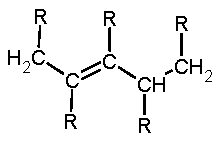
\includegraphics[width=80px]{pent3ene.pdf}
  \caption{Pent-3-ene}
  \label{fig:pent3ene}
\end{subfigure}%
\begin{subfigure}{.3\textwidth}
  \centering
  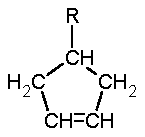
\includegraphics[width=60px]{RcycloPenteneHs.pdf}
  \caption{Cyclo-Pentene}
  \label{fig:cycloPen}
\end{subfigure}
\begin{subfigure}{.3\textwidth}
  \centering
  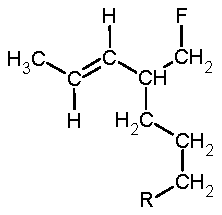
\includegraphics[width=80px]{pent3ene2propNOF.pdf}
  \caption{Pent-3-ene-2-propyl-1-F}
  \label{fig:propSub}
\end{subfigure}
\caption{The chemical structure of molecules in the datasets, R = H, F, OH or NH\textsubscript{2}}
\label{fig:Molecules}
\end{figure}


The following data sets were generated. The first dataset was used for training. The last two datasets were used for testing the robustness. Each configuration in all the datasets will be put under 4 different environments (1 with no environment + 3 different fields for X, Y and Z direction).
\begin{description}
\item[\textit{pent3ene}] This dataset is composed of different derivations of pent-3-ene, as shown in figure~\ref{fig:pent3ene}. The molecule is singly substituted with flourine (-F), hydroxyl (-OH) or amine (-NH\textsubscript{2}) group. Hence the dataset has a set off geometries where each carbon is substituted with each of the 3 subsituents leading to a total of 16 unique molecules including the molecule without any subsituents. This data set has 105 geometry configurations and we split the whole dataset into two parts evenly. We use the first 53 geometries to serve as the training dataset, and the remaining 52 geometries as testing dataset.
\item[\textit{cycloPentene}]Includes singly substituted cyclo-pentene (see figure~\ref{fig:cycloPen}). This data set has 40 geometry configurations.
\item[\textit{pentPropylF}] Includes pent-3-ene-2-propyl-1-Fluorine singly substituted with -F, -OH and -NH\textsubscript{2} (see figure~\ref{fig:propSub}). This data set has 21 geometry configurations.
\end{description}


% DATA SET

We ran the original Hartree-Fock until convergence, so we have the ground truth of the steady-state density matrices and the energy of the given molecular system under different geometries. 
%Since we have the energy of each configuration in the dataset, we can to evaluate the computation time and also the accuracy of the result in each iteration.

% Define error
Our goal is to find a policy which quickly produces a density matrix with low square error. The error is defined as error of matrix + error of energy. The error of the matrix is given by $\|\rho_i-\rho_n\|$. Likewise, the error of energy is given by $|E(\rho_i)-E(\rho_n)|$. Once we have the error function, we can optimize the coefficients by minimizing the square error.

Consequently to prevent the sum of the coefficients to vary too much from 1 a regularization method is implemented which penalizes the model when the sum differs form one. The regularization model included in the optimization is as following:
\[
R =  w [(\sum_i c_i) - 1]
\]
where $w$ is the weight deciding the magnitude of the penalty which was set to 30. This regularization method is added to the minimization of the experts as well as to the DAgger.

% Goal
%The goal is to train the Hartree-Fock with linear combination policy that can reach the steady-state density matrix for a given molecule faster than the original Hartree-Fock.


\subsection{Approach}


In the experiment, we will compare two different policies with baseline. The baseline is the policy that always uses the average of the last two density matrices to serve as the input to the next iteration.
%MENTION THE PURE LINEAR COMBINATION
%In the experiment, we built up two expert's policies.
One naive approach to build the first good policy is always using all the density matrices we have to generate a linear combination that best approaches the final steady-state density matrix after one Hartree-Fock iteration.  For example, from guess density matrix $\rho_0$ we will find the best coefficient that makes the output best approaches the final objective. However, we may get some error thus the result of the first iteration is $\rho_1$.  In the next iteration, again we will try to find the linear combination $(\rho_0, \rho_1)$ that best approaches the final density matrix. We can keep doing this procedure until the output of the Hartree-Fock reaches the final steady-state density matrix.
Because we already know the final steady-state density matrix, and in each iteration we aim for the final objective directly, it's possible that we can build up a trajectory that reaches final density matrix much faster then the original process. At the same time, we will learn a policy from it. Let's call it the ``least squares'' policy.

%SHOULD ALSO MENTIONED TWO DIFFERENT EXPERT \\
Though we already aim for the final objective in each iteration, we still can try to build up a better expert's demonstration from it and perhaps train another policy which is faster than the least squares one.

In the experiment, we built up two different cases of expert's policies. Both are from the trajectory that has a step size of two of the ``least squares'' trajectory. What differs is the initial guess density, one expert policy is the least squares fitting of the process with the initial guess set to zero ($\rho_0 = 0$) and the other expert policy has the initial guess set to an identity matrix ($\rho_0 = I$). Both these experts are aggregated and trained simultaneously in the training of the DAgger model. 

%The other one is from the perfect trajectory which always return the final steady-state matrix in one iteration.

% HOW TO EVALUATE

%MENTION THE CASE THAT MAY NEVER CONVERGE \\
%When iteration of Hartree-Fock converge, we can get the final steady-state density matrix and also the energy of the system. However, the process does not always lead to convergence. For example, under some strong electric fields, the process may keep running and never reach convergence.%

%In the experiment, we will also examine the robustness of different policies by the smoothness of the plot.


%What is convergence rate \\



%CLAIM \\ 
%DAgger tries to learn a new policy by imitating the expert's demonstration. Since the policy space of the DAgger and also the Pure Linear Combination are the same, the result should be at least equal or be better to the Pure Linear Combination trajectory. 
 


\subsection{Experiment result}



\begin{figure}[h!]
\centering
\begin{subfigure}{.5\textwidth}
  \centering
  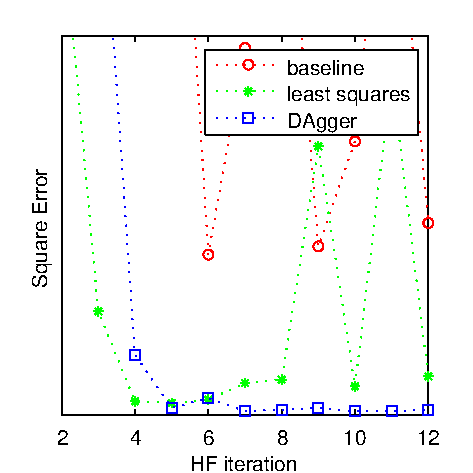
\includegraphics[scale=0.7]{cycloPen_pzero_test_12iter.pdf}
  \caption{$\rho_0 = 0$}
  \label{fig:cycloPen0}
\end{subfigure}%
\begin{subfigure}{.5\textwidth}
  \centering
  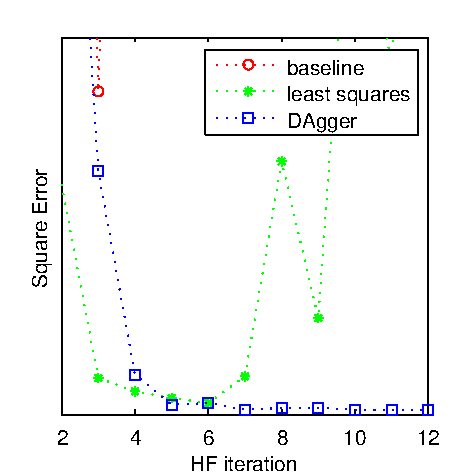
\includegraphics[scale=0.7]{cycloPen_peye_test_12iter.pdf}
  \caption{$\rho_0 = I$}
  \label{fig:cycloPenI}
\end{subfigure}
\caption{Error as a function of iteration tested on \textit{cycloPentene} dataset}
\label{fig:testcycloPen}
\end{figure}

We evaluated the performance of each policy in terms of error and robustness. We will find that least square already converges pretty fast and get much lower error in the same amount of iterations compare to the baseline, since it always tries to reach the final density matrix in each iteration. However, considering DAgger trains on the dataset that aggregates new dataset iteration by iteration. As the dataset growing, it adds more diversity to the dataset and lead to a more robust policy which performs better.

Both the least squares and DAgger converge in just the first few iterations when training on the \textit{pent3ene} dataset. Testing this on the other half of \textit{pent3ene} dataset shows the exact same result and DAgger does not perform better than least squares in each individual case. However, DAgger provides a set of coefficients which lead to convergence within a few steps both for $\rho_0 = 0$ and $\rho_0 = I$.

\begin{figure}[h!]
\centering
\begin{subfigure}{.5\textwidth}
  \centering
  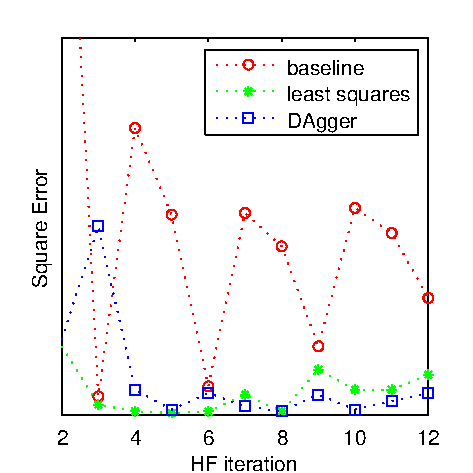
\includegraphics[scale=0.7]{propylsub_pzero_test_12iter.pdf}
  \caption{$\rho_0 = 0$}
  \label{fig:propSub0}
\end{subfigure}%
\begin{subfigure}{.5\textwidth}
  \centering
  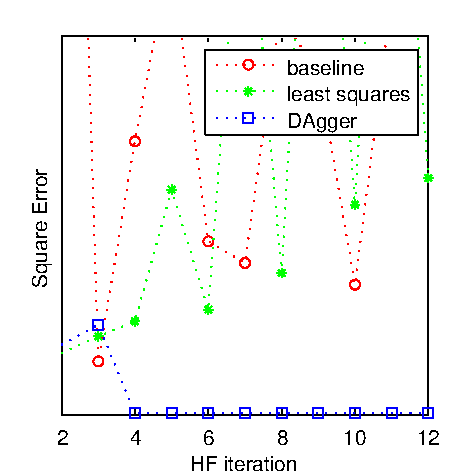
\includegraphics[scale=0.7]{propylsub_peye_test_12iter.pdf}
  \caption{$\rho_0 = I$}
  \label{fig:propSubI}
\end{subfigure}
\caption{Error as a function of iteration tested on \textit{pentPropylF} dataset}
\label{fig:testpropSub}
\end{figure}

Evaluating the robustness of these policies by testing on datasets consisting of different molecules are shown in Figure~\ref{fig:testcycloPen} and \ref{fig:testpropSub}. Least squares does not perform as good as DAgger in these cases, this could be due to tendancy to over-fit. DAgger provides also a more robust set of coefficients given that it is trained on two different initial guess density matrices ($\rho_0 = 0$ and $\rho_0 = I$).



\section{CONCLUSION}
In the experiment, we first proposed the least squares policy. It is easy to train and already can yield much lower error comparing to the baseline. However, it tend to somewhat over-fit the training data and performance fluctuates on testing data accordingly. On the other hand, DAgger does train a more robust policy which is more flexible with input initial guess. DAgger outperforms least squares when tested on different datasets.  
During the training process in DAgger, it keeps aggregating the dataset hence has a more diverse training instances. This can prevent the policy from over-fitting the training dataset thus produces a more stable and smooth decreasing trend. This provides a great property when dealing with large molecules or on the case which is hard to get to convergence.

\bibliography{refs}

\end{document}





%Figure \ref{fig:testZero} shows the error of each policy on the cycloPentene testing dataset for 12 iterations. The baseline is the policy that always uses the average of the last two density matrices to serve as the input to the next iteration.  
%
%We can observe that all the policies seems to converge within 10 iterations except the baseline fluctuates.


%The baseline again fluctuates while all the other policies still converges within 12 iteration. 
%Least squares and DAgger got pretty similar error after 12 iterations.
%
%However, the performance of linear combination fluctuates during iteration 5 - 10 while both DAgger with different experts have a more steady decreasing trend across all 12 iterations. 


%\begin{figure}[h!]
%\center
%  \caption{Absolute value of difference between iterations on training dataset}
%	\label{fig:converge_training}
%    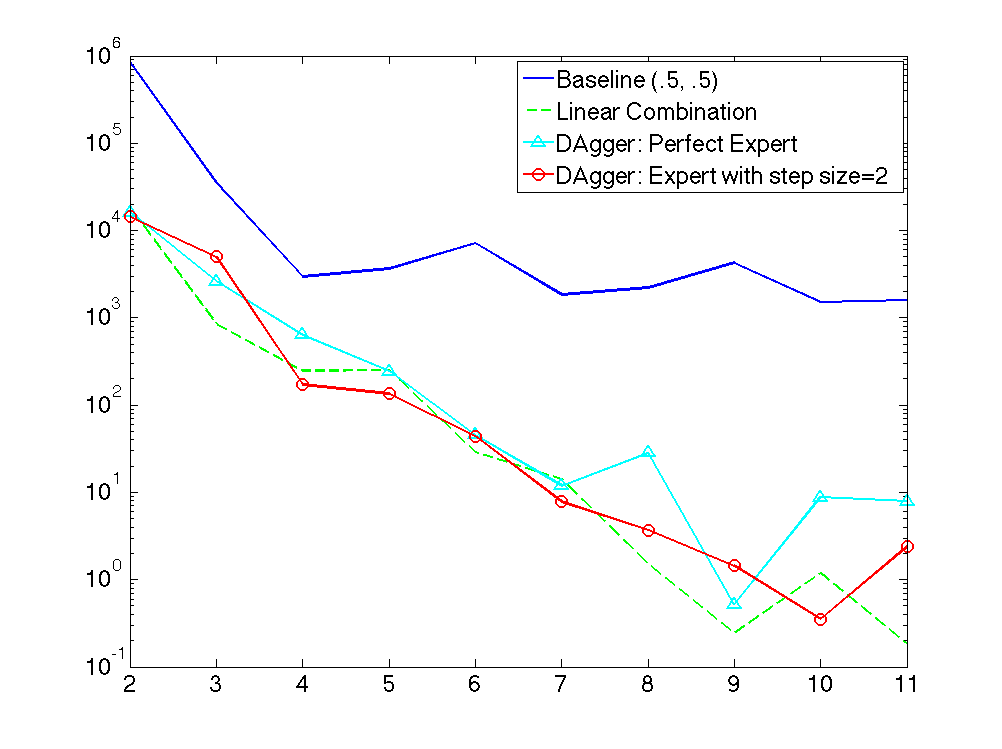
\includegraphics[width=210px]{convergence_Training.png}
%\end{figure}
%
%\begin{figure}[h!]
%\center
%  \caption{Absolute value of difference between iterations on testing dataset}
%  \label{fig:converge_testing}
%    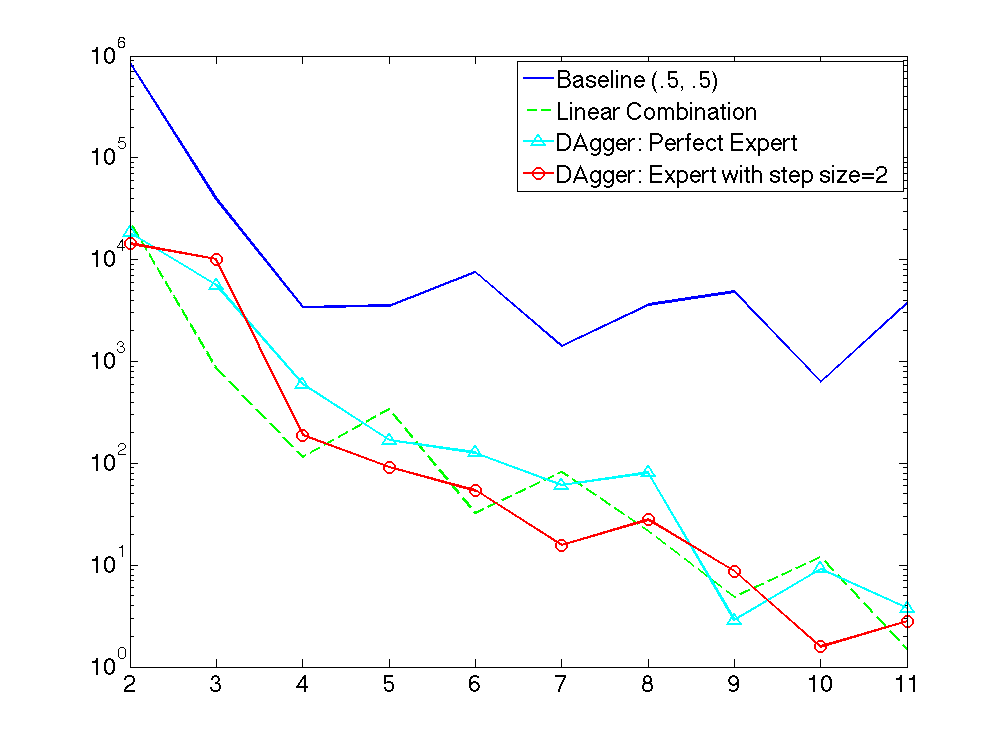
\includegraphics[width=210px]{convergence_Testing.png}
%\end{figure}


%Compare to the result on the training dataset (Figure \ref{fig:training}), the curves are similar for DAgger and baseline, but is pretty different for the least squares. Least squares performs the best and has a smooth result on training dataset while it fluctuates on testing dataset. It is possible because of the least squares over-fit the training dataset. On the contrary, DAgger with the expert that has step size of 2 got more consistent results between training and testing dataset.
%
%

%\begin{figure}[h!]
%\centering
%\begin{subfigure}{.5\textwidth}
%  \centering
%  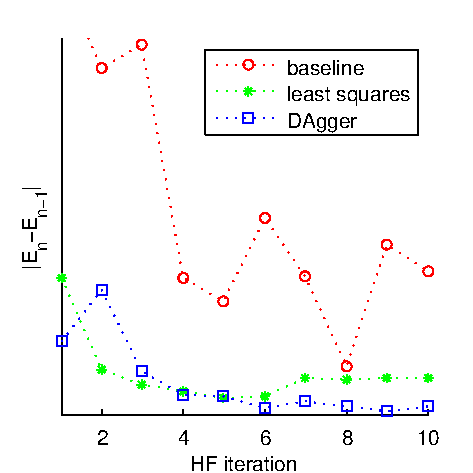
\includegraphics[scale=0.7]{dE_cycloPen_pzero_test_12iter.pdf}
%  \caption{$\rho_0 = 0$}
%  \label{fig:sub1}
%\end{subfigure}%
%\begin{subfigure}{.5\textwidth}
%  \centering
%  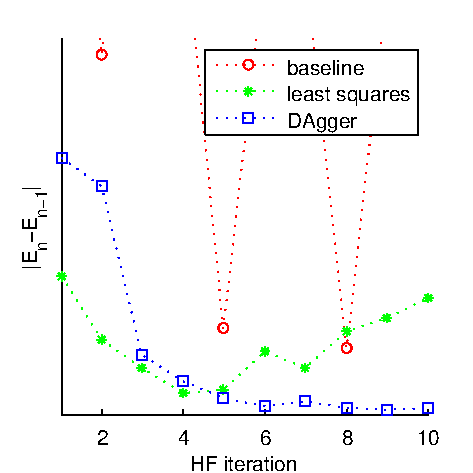
\includegraphics[scale=0.7]{dE_cycloPen_peye_test_12iter.pdf}
%  \caption{$\rho_0 = I$}
%  \label{fig:sub2}
%\end{subfigure}
%\caption{Error as a function of iteration for test on \textit{cycloPentene} dataset}
%\label{fig:test}
%\end{figure}